	\section{Цель работы}
		Решение 2х-мерной задачи симуляции жидкости (газа) методом решеточных уравнений Больцмана.
		
		Матрица задачи должна занимать в памяти не менее 100 Мб на каждое процессорное ядро, задействованное в вычислениях, верхний предел – 1Гб на ядро. По возможности использовать при решении специализированные функции MPI: $ MPI\_Sendrecv\_replace $, $  MPI\_Reduce $.
	\section{Порядок выполенения работы}
	
		\subsection{Описание алгоритма}
			
			\begin{figure}[h]
				\centering
				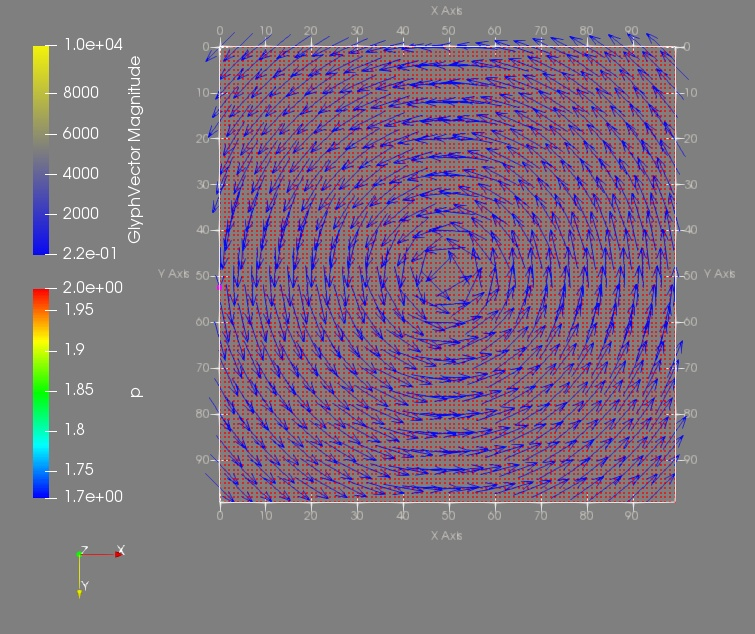
\includegraphics[width=\linewidth]{0000}
				\caption[Начальные условия]{}
				\caption{}
				\label{fig:start}
			\end{figure}
			\begin{figure}[h]
				\centering
				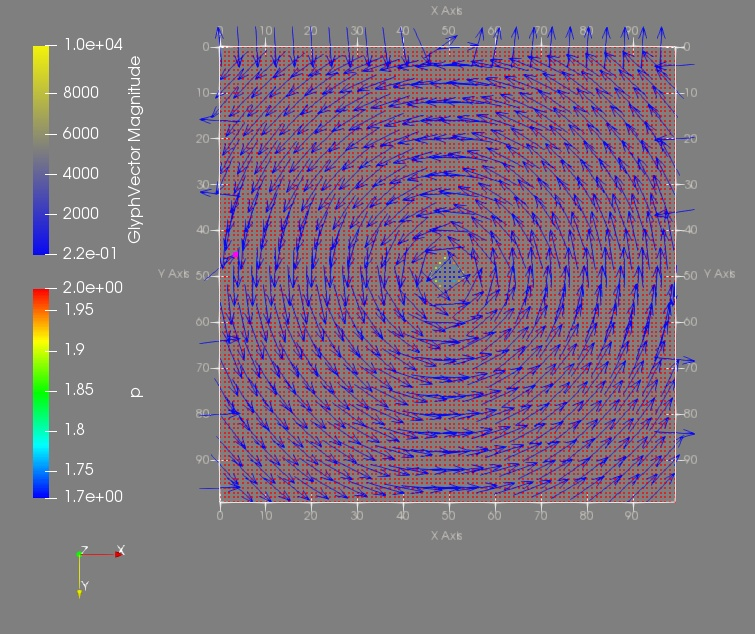
\includegraphics[width=\linewidth]{0001}
				\caption{}
				\label{fig:asd}
			\end{figure}
			\begin{figure}[h]
				\centering
				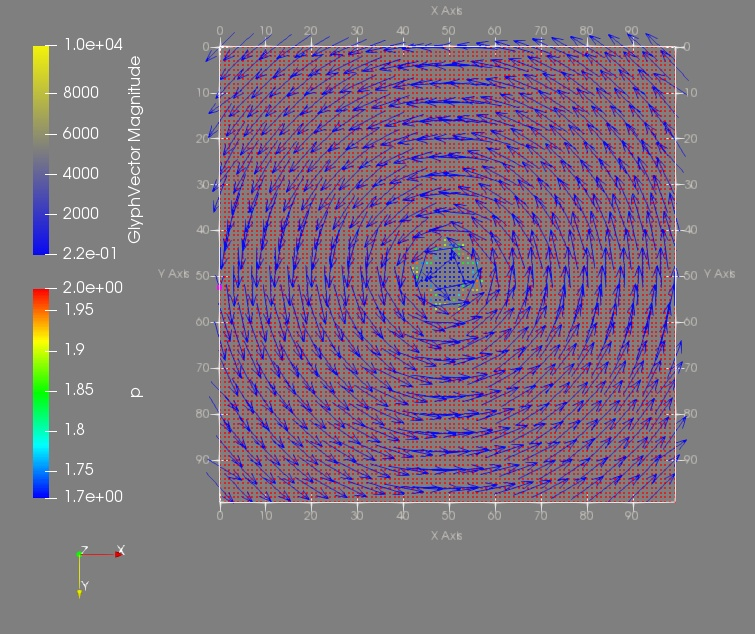
\includegraphics[width=\linewidth]{0002}
				\caption{}
				\label{fig:asd}
			\end{figure}
			\begin{figure}[h]
				\centering
				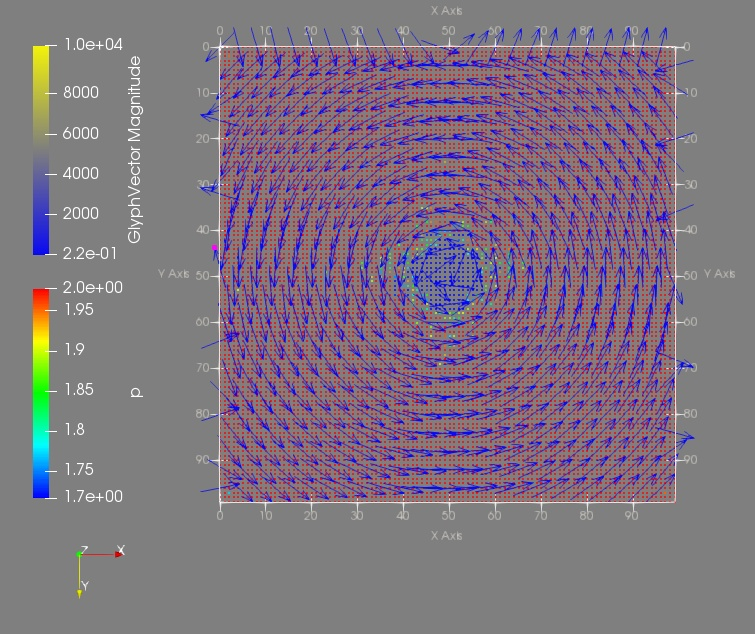
\includegraphics[width=\linewidth]{0003}
				\caption{}
				\label{fig:1}
			\end{figure}
			\begin{figure}[h]
				\centering
				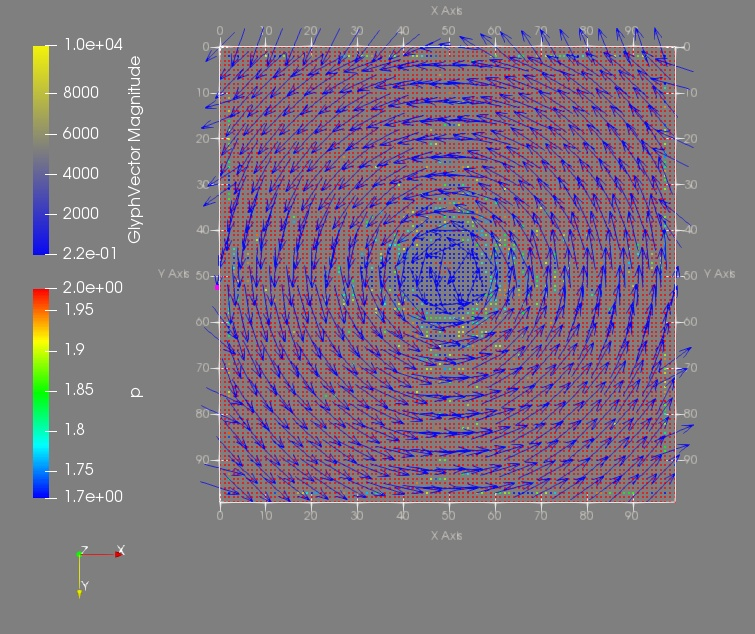
\includegraphics[width=\linewidth]{0004}
				\caption{}
				\label{fig:asd}
			\end{figure}
			\begin{figure}[h]
				\centering
				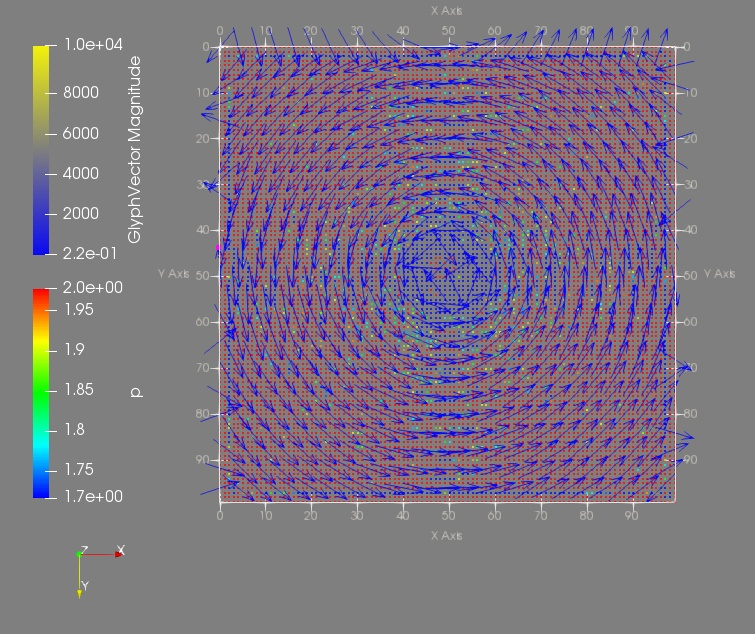
\includegraphics[width=\linewidth]{0005}
				\caption{}
				\label{fig:asd}
			\end{figure}
			\begin{figure}[h]
				\centering
				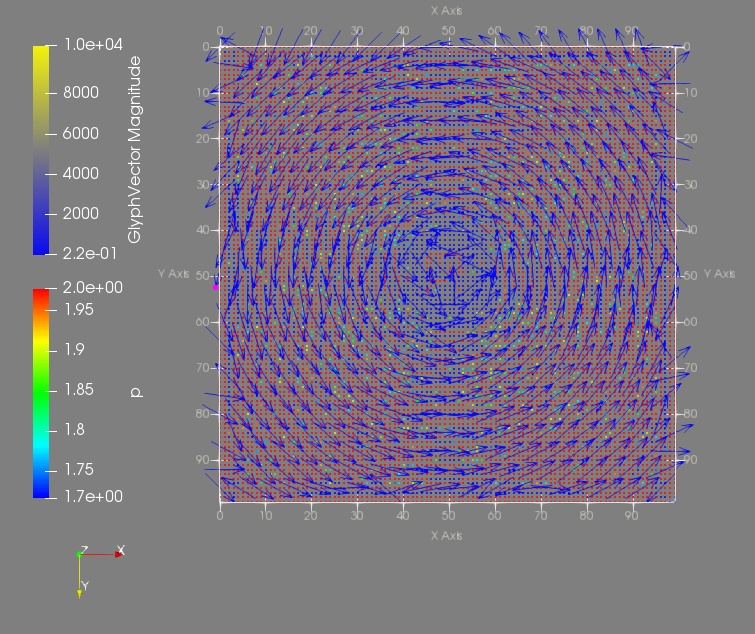
\includegraphics[width=\linewidth]{0006}
				\caption{}
				\label{fig:asd}
			\end{figure}
			\begin{figure}[h]
				\centering
				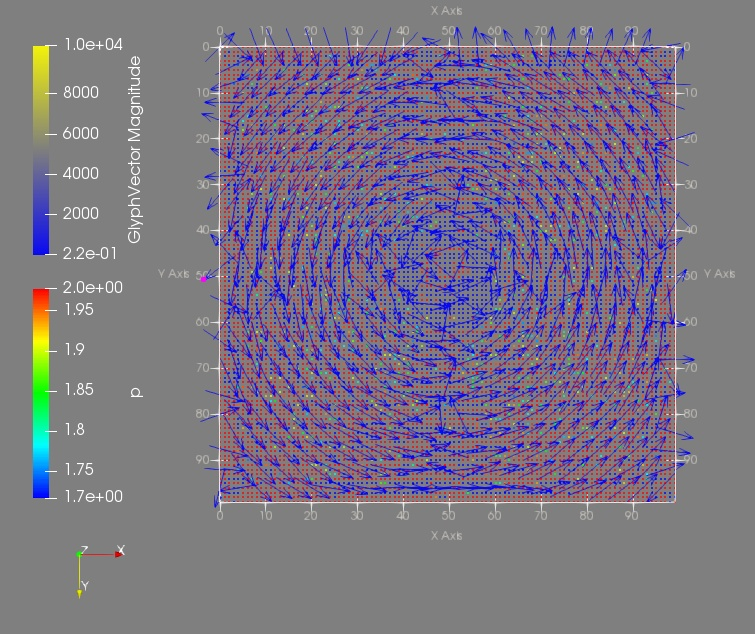
\includegraphics[width=\linewidth]{0007}
				\caption{}
				\label{fig:asd}
			\end{figure}

		\subsection{Методика распараллеливания}
			Узел с нулевым индексом (далее главный) генерирует равный объём данных и рассылает поочерёдно всем остальным узлам. Далее главный узел сгенерирует вектор результатов.
			
			Далее в каждом столбце происходит поиск максимального элемента на главной диагонали и ниже. Если он лежит не на главной диагонали, все узлы меняют строку с максимумом со строкой главной диагонали.
			
			На активном узле происходит подсчёт множителей по методу Гаусса, а потом широковещательным сообщением множители отправляются остальным узлам и выполняется приращение по методу Гаусса.
			
		\subsection{Исследование производительности реализованного алгоритма}
			
			Метод Гаусса требует $ O(n^3) $ арифметических операций. Тогда производительность метода можно оценить формулой $ n^3/\tau $, где $ \tau $ - время выполнения алгоритма. На основе таблицы результатов \ref{t1} составлен график зависимости производительности от количества процессоров \ref{fig:performance}. 
			
			Как видно из графика \ref{fig:performance}, увеличение производительности с ростом количества процессоров близко к линейному.
			
		
			\begin{table}
				\centering
				\caption{Результаты вычислений, где $ P $ - количество процессоров, $ n $ - размер системы уравнений, $ \tau $ - время выполнения}
				\label{t1}
				\csvreader[tabular=|l|r|l|c|,
				table head=\hline & P & n & $ \tau $\\\hline,
				late after line=\\\hline]%
				{listings/data.csv}{numberOfProcessors=\pnumber,equationCount=\n,allRounds=\ftime}%
				{\thecsvrow & \pnumber& \n & \ftime }%
			\end{table}
			\begin{figure}
				\centering
				\begin{tikzpicture}
					\begin{axis}[ylabel=Производительность оп/сек., xlabel=Количество процессоров, xtick={0,3,6,9,12,16,20,24,28,32}]
						\addplot table [x=numberOfProcessors, y expr=\thisrow{equationCount}^3/(\thisrow{allRounds}), col sep=comma] {listings/data.csv};
%						\addplot table [x=numberOfProcessors, y={create col/linear regression={y=equationCount}, col sep=comma] {listings/data.csv};
					\end{axis}
				\end{tikzpicture}
				\caption{Зависимость производительности алгоритма от количества процессоров.} \label{fig:performance}
			\end{figure}
				
	\section{Вывод}
		В ходе работы
		\begin{enumerate}
			\item Реализован алгоритм Гаусса с выбором главного элемента в столбце с задаными ограничениями на начальные данные.
			\item Проанализирована производительность алгоритма.
		\end{enumerate}
	
		Исходный код программ доступен по ссылке \href{https://github.com/goto1134/MPI-labs}{https://github.com/goto1134/MPI-labs}.